\documentclass[12pt,a4paper]{article}

\usepackage[utf8]{inputenc}
\usepackage[T1]{fontenc}
\usepackage[brazil]{babel}
\usepackage{geometry}
\usepackage{booktabs}
\usepackage{array}
\usepackage{longtable}
\usepackage{float}
\usepackage{hyperref}
\usepackage{amsmath}a
\usepackage{graphicx}

\geometry{margin=2.5cm}

\title{Predição de Preços de Imóveis em Fortaleza com Modelos de Aprendizagem de Máquina}
\author{Tiago Oliveira Lima \\ Noberto Frota Oliveira Nogueira \\ Luzia Vitória Freitas Loiola}
\date{\today}

\begin{document}

\maketitle

\begin{abstract}
Este trabalho apresenta o desenvolvimento e a avaliação de uma solução de aprendizagem de máquina para predição de preços de imóveis residenciais na cidade de Fortaleza, Ceará. O problema foi formulado como uma tarefa de regressão supervisionada, na qual atributos físicos, locacionais e de infraestrutura do imóvel são usados para estimar o valor de venda anunciado. A base de dados foi construída a partir de dados obtidos por web scraping, seguida por uma etapa de tratamento, padronização de variáveis e remoção de registros inconsistentes. Foram avaliados modelos baseados em árvores, com destaque para CatBoost, XGBoost, LightGBM e Random Forest, além de modelos lineares, SVM e redes neurais na estrutura geral da pipeline. O principal experimento com busca bayesiana de hiperparâmetros, usando Optuna e validação cruzada, indicou melhor desempenho para o XGBoost, com RMSE de R\$ 414.288,80, MAE de R\$ 232.003,72 e $R^2$ de 0,7236. Os resultados mostram que modelos de árvores são adequados para dados tabulares heterogêneos do mercado imobiliário e capturam melhor as relações não lineares entre localização, área, características do imóvel e preço.
\end{abstract}

\section{Introdução}

A precificação de imóveis é uma tarefa relevante para compradores, vendedores, corretores, incorporadoras e plataformas digitais de anúncios. Em centros urbanos, o preço de um imóvel não depende apenas de sua área ou número de quartos, mas também de fatores como bairro, padrão do empreendimento, proximidade de regiões valorizadas, vagas de garagem, infraestrutura do condomínio e atributos de lazer. Essa combinação de fatores torna o problema naturalmente não linear e sujeito a variações de mercado ao longo do tempo.

O projeto desenvolvido tem como objetivo construir uma plataforma de predição de preços de imóveis em Fortaleza, Ceará, usando dados atualizados extraídos por web scraping. A solução proposta é composta por uma pipeline de dados, uma pipeline de modelos, uma API e uma interface de usuário. A pipeline de dados recebe dados brutos de anúncios, realiza tratamento e padronização, e disponibiliza registros consistentes para treinamento. A pipeline de modelos treina diferentes algoritmos candidatos, seleciona o melhor modelo e persiste o artefato campeão para uso em predições. A API expõe endpoints para inserção de dados, treinamento e predição, enquanto a interface permite ao usuário informar as características de um imóvel e receber uma estimativa de preço.

Do ponto de vista de aprendizagem de máquina, o problema foi definido como uma tarefa de regressão supervisionada, pois a variável alvo é contínua: o preço do imóvel. A motivação principal é investigar quais modelos conseguem representar melhor a estrutura do mercado imobiliário local e produzir estimativas úteis a partir de dados tabulares reais, ruidosos e heterogêneos.

\section{Fundamentação Teórica}

\subsection{Problema de regressão imobiliária}

Modelos hedônicos de preço são amplamente usados para estimar o valor de bens imóveis a partir de seus atributos observáveis. Nessa abordagem, o preço é interpretado como resultado da combinação de características internas do imóvel, como área e quantidade de cômodos, e características externas, como localização e infraestrutura urbana. Em termos de aprendizagem supervisionada, dado um conjunto de observações $(x_i, y_i)$, em que $x_i$ representa os atributos de um imóvel e $y_i$ seu preço, busca-se aprender uma função $f(x)$ capaz de aproximar o valor esperado do preço.

Embora modelos lineares sejam úteis como referência, o mercado imobiliário apresenta relações que dificilmente seguem uma única tendência linear. Por exemplo, a primeira vaga de garagem pode gerar um ganho de valor maior do que vagas adicionais, a valorização por bairro pode ocorrer em patamares discretos, e imóveis de luxo podem atuar como outliers. Por isso, modelos baseados em árvores de decisão e ensembles tendem a ser competitivos em dados tabulares, pois conseguem particionar o espaço de atributos por regras condicionais e capturar interações complexas entre variáveis.

\subsection{Descrição dos dados}

A base tratada utilizada no principal notebook de modelagem contém 3.711 registros válidos e 19 atributos de entrada, além da variável alvo \texttt{preco}. Os dados representam imóveis residenciais anunciados em Fortaleza e incluem apartamentos, casas, coberturas, studios e imóveis duplex ou triplex. A Tabela~\ref{tab:features} resume as variáveis usadas nos modelos.

\begin{table}[H]
\centering
\caption{Conjunto de atributos utilizados na modelagem.}
\label{tab:features}
\begin{tabular}{p{4cm} p{10cm}}
\toprule
Tipo & Variáveis \\
\midrule
Locacionais e categóricas & \texttt{bairro}, \texttt{tipo\_imovel\_padronizado} \\
Numéricas & \texttt{area\_m2}, \texttt{quartos}, \texttt{banheiros}, \texttt{suites}, \texttt{andar}, \texttt{vagas} \\
Booleanas de infraestrutura & \texttt{portaria}, \texttt{vista\_mar}, \texttt{condominio\_fechado}, \texttt{piscina}, \texttt{deck}, \texttt{varanda}, \texttt{academia}, \texttt{salao\_festa}, \texttt{salao\_jogos}, \texttt{quadra\_campo} \\
Alvo & \texttt{preco} \\
\bottomrule
\end{tabular}
\end{table}

Nos experimentos do notebook \texttt{modelagem\_busca\_bayesiana.ipynb}, também foi considerada a variável \texttt{varanda\_gourmet}, totalizando 19 features. Na implementação da API, o contrato final de predição usa 18 atributos, sem \texttt{varanda\_gourmet}. Essa diferença reflete uma evolução entre o ambiente experimental e a versão operacional da pipeline.

A Tabela~\ref{tab:estatisticas} apresenta estatísticas descritivas da base tratada usada nos experimentos. Observa-se grande dispersão no preço, o que reforça a necessidade de métricas capazes de penalizar erros elevados e de modelos robustos a outliers.

\begin{table}[H]
\centering
\caption{Estatísticas descritivas das principais variáveis numéricas.}
\label{tab:estatisticas}
\begin{tabular}{lrrrrr}
\toprule
Variável & Média & Mediana & Desvio padrão & Mínimo & Máximo \\
\midrule
\texttt{preco} & 911.016,70 & 692.513,00 & 788.643,40 & 33.000,00 & 7.800.000,00 \\
\texttt{area\_m2} & 155,46 & 123,00 & 112,02 & 10,00 & 810,00 \\
\texttt{quartos} & 3,17 & 3,00 & 1,04 & 1,00 & 13,00 \\
\texttt{banheiros} & 3,30 & 3,00 & 1,42 & 1,00 & 15,00 \\
\texttt{suites} & 2,35 & 2,00 & 1,13 & 1,00 & 11,00 \\
\texttt{andar} & 1,51 & 0,00 & 4,05 & 0,00 & 50,00 \\
\texttt{vagas} & 2,55 & 2,00 & 1,63 & 0,00 & 12,00 \\
\bottomrule
\end{tabular}
\end{table}

Os bairros mais frequentes na base foram Aldeota, Meireles, Engenheiro Luciano Cavalcante, Cocó e Edson Queiroz. Em relação ao tipo de imóvel, a base é composta majoritariamente por \texttt{apartamento\_padrao} e \texttt{casa\_padrao}. A presença do bairro como variável categórica é importante porque o mercado imobiliário atribui valor ao nome da região, não apenas às coordenadas geográficas. Dois imóveis próximos podem ter preços diferentes por pertencerem a bairros com percepção de status distinta. Além disso, árvores de decisão trabalham por cortes ortogonais; usar somente latitude e longitude exigiria muitas divisões para aproximar contornos urbanos reais, aumentando o risco de sobreajuste.

\subsection{Modelos relacionados}

Foram considerados algoritmos clássicos e modernos de regressão. Modelos lineares com regularização, como Ridge e Lasso, serviram como referência pela simplicidade e interpretabilidade. O SVR permite capturar relações não lineares por meio de kernels, mas pode ter maior custo computacional e sensibilidade à escala. Redes neurais do tipo MLP também foram avaliadas como alternativa flexível, embora geralmente exijam mais dados e ajuste cuidadoso para superar ensembles em dados tabulares.

Os modelos que receberam maior atenção foram os baseados em árvores: Random Forest, XGBoost, LightGBM e CatBoost. O Random Forest combina múltiplas árvores treinadas sobre amostras e subconjuntos de variáveis, reduzindo variância. XGBoost e LightGBM são métodos de gradient boosting, nos quais árvores são adicionadas sequencialmente para corrigir erros dos modelos anteriores. O CatBoost também é um método de boosting, com tratamento eficiente de variáveis categóricas e estratégias para reduzir viés em sua codificação. Esses modelos são adequados ao problema por lidarem bem com dados tabulares mistos, relações de limiar e outliers.

\section{Metodologia}

\subsection{Pipeline de dados}

Os dados brutos são provenientes de scraping de anúncios imobiliários. A etapa de tratamento padroniza o esquema de entrada, normaliza nomes de bairros e tipos de imóveis, converte variáveis booleanas de infraestrutura, valida cidade e tipo residencial, calcula variáveis auxiliares como preço por metro quadrado e remove registros inconsistentes. Entre os filtros aplicados estão deduplicação por identificador ou conteúdo, remoção de imóveis não residenciais, cortes de outliers por quantis, remoção de registros sem preço ou metragem e validação de features essenciais.

Na arquitetura da plataforma, os dados tratados são persistidos em PostgreSQL com \texttt{data\_salvamento}. Essa data permite que a pipeline de modelos utilize apenas registros do último ano, reduzindo o impacto de preços defasados sobre a qualidade do modelo. Para os experimentos de notebook, os dados tratados foram lidos de arquivos CSV versionados no repositório.

\subsection{Pré-processamento}

O pré-processamento foi implementado com \texttt{ColumnTransformer}. As variáveis numéricas foram imputadas pela mediana e normalizadas com \texttt{StandardScaler}. As variáveis categóricas foram imputadas pelo valor mais frequente e codificadas com \texttt{OneHotEncoder}, usando \texttt{handle\_unknown="ignore"} para permitir bairros ou tipos não vistos durante o treinamento. As variáveis booleanas foram repassadas diretamente ao modelo.

Esse fluxo garante que modelos sensíveis à escala, como SVR, MLP e modelos lineares, recebam entradas adequadas, ao mesmo tempo em que mantém uma representação compatível com modelos de árvore. Na implementação operacional, o CatBoost também pode usar tratamento nativo para variáveis categóricas.

\subsection{Treinamento e seleção}

A pipeline de modelos foi organizada para treinar diferentes famílias de algoritmos e selecionar o campeão pelo menor RMSE. O registro de modelos da API inclui XGBoost, LightGBM, CatBoost, Random Forest, Ridge, Lasso, SVR e MLP. O notebook principal de experimentos concentrou-se em CatBoost, XGBoost, Random Forest e LightGBM, pois os testes preliminares indicaram que os modelos baseados em árvores apresentavam desempenho superior e mais homogêneo.

Para busca de hiperparâmetros, foi utilizada otimização bayesiana com Optuna. Diferentemente de um grid search exaustivo, a busca bayesiana usa o histórico das tentativas anteriores para priorizar regiões promissoras do espaço de hiperparâmetros. Em cada tentativa, os parâmetros sugeridos foram avaliados por validação cruzada K-Fold com três divisões, embaralhamento e semente aleatória fixa. O objetivo de otimização foi minimizar o RMSE médio nos folds.

\subsection{Métricas de avaliação}

Foram usadas três métricas principais:

\begin{equation}
MAE = \frac{1}{n}\sum_{i=1}^{n}|y_i - \hat{y}_i|
\end{equation}

\begin{equation}
RMSE = \sqrt{\frac{1}{n}\sum_{i=1}^{n}(y_i - \hat{y}_i)^2}
\end{equation}

\begin{equation}
R^2 = 1 - \frac{\sum_{i=1}^{n}(y_i - \hat{y}_i)^2}{\sum_{i=1}^{n}(y_i - \bar{y})^2}
\end{equation}

O MAE representa o erro absoluto médio em reais, sendo de fácil interpretação para o negócio. O RMSE também é expresso em reais, mas penaliza mais fortemente grandes erros, o que é importante em um domínio com imóveis de alto valor. O $R^2$ mede a proporção da variabilidade do preço explicada pelo modelo.

\section{Experimentos}

\subsection{Configuração experimental}

O experimento principal foi executado no notebook \texttt{modelagem\_busca\_bayesiana.ipynb}. A base utilizada foi \texttt{dados\_tratados/dados\_tratados/imoveis\_tratado.csv}, após remoção de registros com valores ausentes nas features obrigatórias e no alvo. O conjunto final teve 3.711 imóveis válidos. Foram usados 50 trials de Optuna por modelo, validação cruzada K-Fold com três folds e semente aleatória 42.

Os modelos comparados no notebook foram:

\begin{itemize}
    \item CatBoost;
    \item XGBoost;
    \item Random Forest;
    \item LightGBM.
\end{itemize}

Cada modelo recebeu um espaço próprio de hiperparâmetros. Em seguida, o melhor conjunto de parâmetros foi usado para ajustar o modelo final e salvar os artefatos. O notebook também produziu curvas de convergência da busca bayesiana, gráficos comparativos de RMSE e $R^2$, gráfico de valores reais versus previstos e análise visual de resíduos. Esses elementos foram usados não apenas para escolher o menor erro médio, mas também para verificar estabilidade da busca, proximidade entre os modelos líderes e comportamento dos erros ao longo da faixa de preços.

\subsection{Resultados do experimento bayesiano}

A Tabela~\ref{tab:ranking-notebook} apresenta o ranking obtido no notebook. O XGBoost obteve o menor RMSE, com desempenho muito próximo ao LightGBM. A diferença entre os dois primeiros foi inferior a R\$ 700 em RMSE, o que indica empate técnico considerando a escala dos preços. CatBoost e Random Forest também apresentaram resultados competitivos, mas com erros um pouco maiores.

\begin{table}[H]
\centering
\caption{Ranking do experimento com busca bayesiana e K-Fold.}
\label{tab:ranking-notebook}
\begin{tabular}{lrrr}
\toprule
Modelo & RMSE (R\$) & MAE (R\$) & $R^2$ \\
\midrule
XGBoost & 414.288,80 & 232.003,72 & 0,7236 \\
LightGBM & 414.976,29 & 234.524,12 & 0,7227 \\
CatBoost & 422.171,53 & 234.471,00 & 0,7133 \\
Random Forest & 431.852,03 & 236.597,69 & 0,6999 \\
\bottomrule
\end{tabular}
\end{table}

O resultado confirma a hipótese de que modelos de árvores são adequados ao problema. O preço de imóveis depende de interações como bairro e área, tipo de imóvel e vagas, ou presença de infraestrutura e padrão do empreendimento. Esses efeitos aparecem em patamares e combinações condicionais, sendo melhor representados por árvores do que por uma única superfície linear.

A Figura~\ref{fig:comparacao-modelos} apresenta visualmente a comparação entre os quatro modelos avaliados. O XGBoost obteve o menor RMSE e o maior $R^2$, mas a diferença para o LightGBM foi pequena: apenas R\$ 687,50 de RMSE e 0,0009 ponto de $R^2$. Essa proximidade caracteriza um empate técnico entre os dois modelos líderes. O CatBoost ficou em terceiro lugar, ainda com desempenho competitivo, enquanto o Random Forest apresentou o maior erro e o menor $R^2$ entre os modelos baseados em árvores.

\begin{figure}[H]
\centering
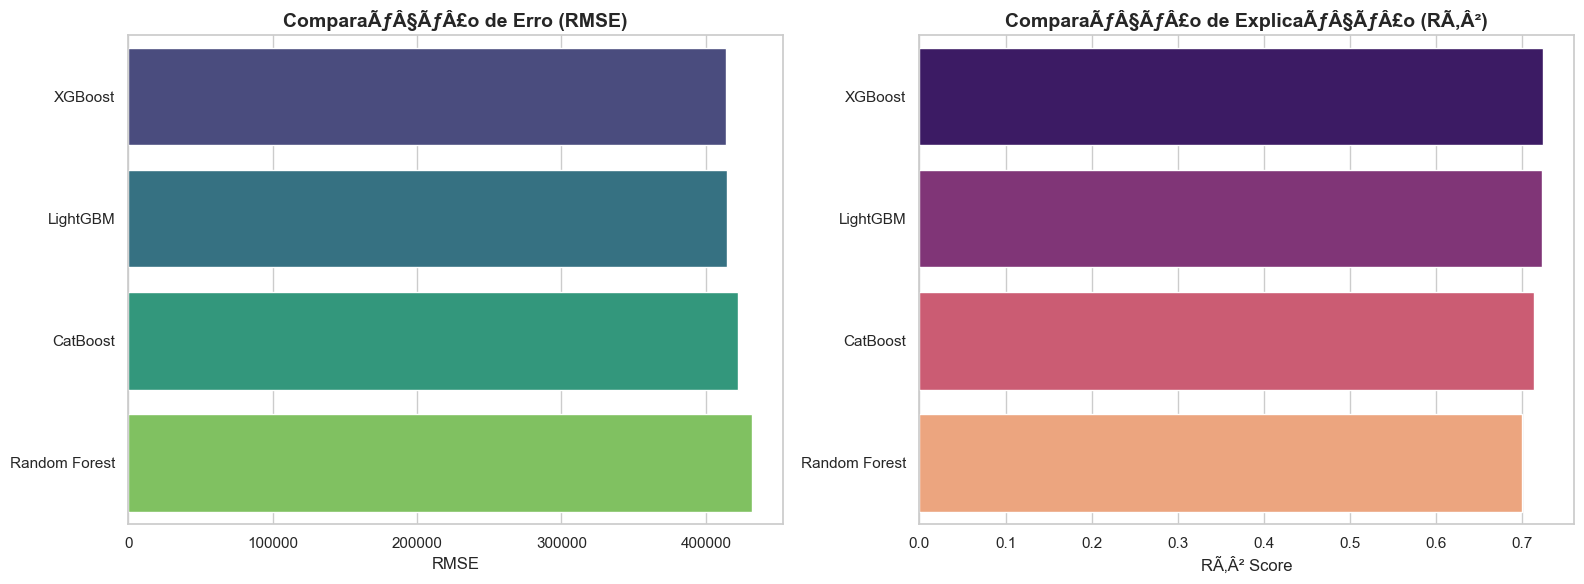
\includegraphics[width=\textwidth]{figures/comparacao_modelos.png}
\caption{Comparação dos modelos por RMSE e $R^2$ no experimento bayesiano.}
\label{fig:comparacao-modelos}
\end{figure}

As curvas e gráficos do notebook indicam que as melhores configurações foram encontradas ao longo das tentativas do Optuna e que os ganhos passam a ser marginais para os modelos líderes. Esse comportamento sugere que o espaço de busca definido foi suficiente para encontrar regiões competitivas de hiperparâmetros, especialmente para XGBoost, LightGBM e CatBoost. A decisão operacional entre XGBoost e LightGBM deve considerar não apenas RMSE, mas também tempo de treinamento, estabilidade em retreinos, facilidade de implantação e interpretabilidade das importâncias de variáveis.

\subsection{Discussão dos resultados}

O melhor desempenho do XGBoost no notebook pode ser explicado por sua capacidade de controlar viés e variância por meio de boosting, regularização, amostragem de linhas e colunas, profundidade máxima e taxa de aprendizado. O LightGBM apresentou desempenho praticamente equivalente, mostrando que métodos de gradient boosting são muito adequados para a estrutura da base. O CatBoost, apesar de não ter vencido o experimento, manteve resultado próximo aos líderes, o que indica robustez e competitividade, especialmente em cenários com variáveis categóricas relevantes como bairro e tipo de imóvel.

O Random Forest teve desempenho inferior aos modelos de boosting, mas ainda forte. Como suas árvores são treinadas de forma mais independente, ele reduz variância, porém tende a ter menor capacidade de correção sequencial de erros em comparação com boosting. A diferença observada entre Random Forest e os modelos de boosting reforça a vantagem de algoritmos que ajustam novas árvores de forma direcionada aos erros anteriores.

A Figura~\ref{fig:real-previsto} mostra o diagnóstico de valores reais versus previstos para o melhor modelo. A nuvem de pontos acompanha a diagonal de predição perfeita, principalmente para imóveis até aproximadamente R\$ 3 milhões. Isso indica que o modelo aprendeu a tendência central dos preços e apresenta boa calibração geral. Entretanto, em imóveis de maior valor, a dispersão aumenta e aparecem casos em que o modelo subestima imóveis caros, comportamento esperado em bases com poucos exemplos de alto padrão e maior variância de preço.

\begin{figure}[H]
\centering
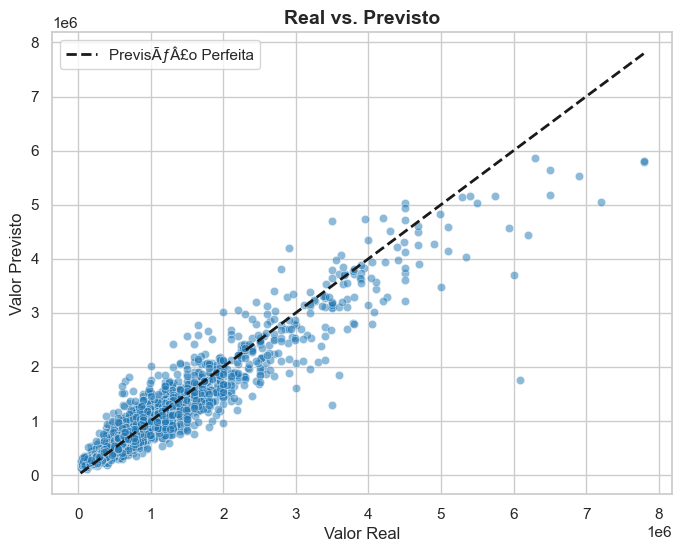
\includegraphics[width=0.78\textwidth]{figures/real_vs_previsto.png}
\caption{Valores reais versus valores previstos pelo melhor modelo do experimento.}
\label{fig:real-previsto}
\end{figure}

A distribuição dos resíduos, apresentada na Figura~\ref{fig:distribuicao-residuos}, é concentrada ao redor de zero, indicando que a maior parte das predições possui erro moderado. Ao mesmo tempo, há cauda à direita, o que significa que alguns imóveis tiveram preço real maior que o previsto. Em outras palavras, o modelo tende a errar mais em alguns imóveis caros ou atípicos, principalmente por subestimação.

\begin{figure}[H]
\centering
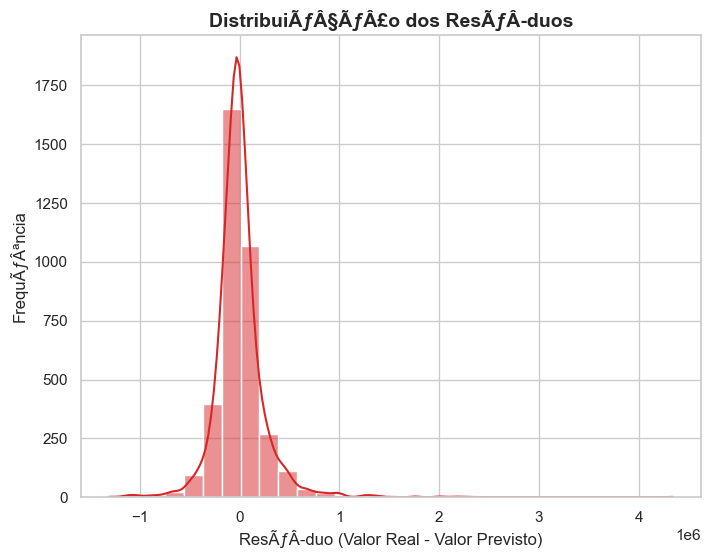
\includegraphics[width=0.78\textwidth]{figures/distribuicao_residuos.png}
\caption{Distribuição dos resíduos do melhor modelo.}
\label{fig:distribuicao-residuos}
\end{figure}

A Figura~\ref{fig:residuos-previstos} reforça essa leitura. Para valores previstos menores, os resíduos ficam mais concentrados em torno da linha zero. À medida que o valor previsto cresce, a amplitude dos resíduos aumenta, evidenciando heterocedasticidade: o erro absoluto tende a ser maior em imóveis mais caros. Uma investigação futura poderia avaliar transformação logarítmica do alvo, segmentação por tipo de imóvel ou modelos especializados por faixa de preço para reduzir esse efeito.

\begin{figure}[H]
\centering
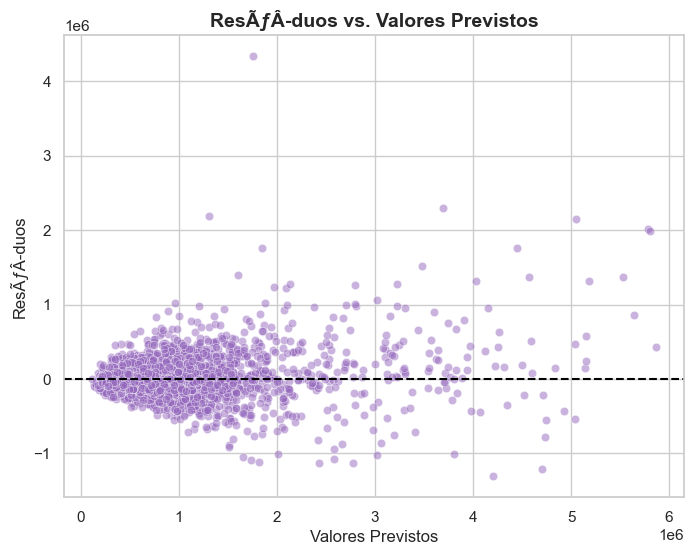
\includegraphics[width=0.78\textwidth]{figures/residuos_vs_previstos.png}
\caption{Resíduos em função dos valores previstos.}
\label{fig:residuos-previstos}
\end{figure}

\subsection{Integração com a plataforma}

Além dos experimentos, o repositório implementa uma API com os endpoints principais do sistema. O endpoint \texttt{/insertData} recebe CSVs de dados brutos, executa a pipeline de tratamento e salva os registros tratados. O endpoint \texttt{/trainModels} cria um experimento de treinamento, carrega dados ativos do último ano, executa a busca de modelos e ativa automaticamente o campeão. O endpoint \texttt{/predict} recebe as características de um imóvel e retorna o preço estimado pelo modelo ativo.

A plataforma também contém um indicador simples de drift em \texttt{/model-health/drift}. A lógica atual compara o preço médio dos imóveis salvos nos últimos 30 dias com o preço médio da base anterior. Se houver menos de 20 amostras recentes, o status é amarelo por baixa volumetria. Se a variação absoluta do preço médio for maior ou igual a 20\%, o status é vermelho; se for maior ou igual a 10\%, o status é amarelo; caso contrário, o status é verde. Esse mecanismo funciona como um sinal prático de mudança de mercado, embora ainda não substitua testes estatísticos de drift por feature, como PSI, teste KS ou distância de Wasserstein.

\section{Conclusão}

Este trabalho desenvolveu e avaliou uma solução de aprendizagem de máquina para predição de preços de imóveis em Fortaleza. O problema foi formulado como regressão supervisionada, usando dados tabulares obtidos por scraping e tratados por uma pipeline específica para o domínio imobiliário. Os experimentos mostraram que modelos baseados em árvores, especialmente XGBoost, LightGBM, CatBoost e Random Forest, são mais adequados que modelos lineares, SVR e MLP para este conjunto de dados.

No experimento principal com busca bayesiana, o XGBoost obteve o melhor desempenho, com RMSE de R\$ 414.288,80, MAE de R\$ 232.003,72 e $R^2$ de 0,7236. O LightGBM ficou praticamente empatado, com RMSE de R\$ 414.976,29 e $R^2$ de 0,7227. A diferença pequena entre XGBoost, LightGBM e CatBoost indica que a seleção final do modelo pode variar conforme atualização da base, espaço de hiperparâmetros e critérios operacionais.

Como trabalhos futuros, recomenda-se avaliar transformação logarítmica do preço, enriquecer as variáveis geográficas com distâncias a pontos de interesse, testar modelos por segmento de imóvel, implementar testes estatísticos de drift por feature, ampliar a validação temporal para simular dados futuros e fortalecer a explicabilidade das predições. Também é importante consolidar a integração da pipeline com PostgreSQL e automatizar rotinas de monitoramento, retreinamento e comparação histórica de modelos.

\section{Contribuição dos Participantes}

A elaboração da plataforma, modelagem e documentação deste projeto ocorreu de forma colaborativa, com a seguinte divisão de responsabilidades:

\begin{itemize}
    \item \textbf{Tiago Oliveira Lima:} Responsável pela modelagem, decisão dos modelos que seriam utilizados, implementação de algoritmos de predição (Random Forest, XGBoost, rede neural, SVR, MLPRegressor e CatBoost), implementação da pipeline de dados, implementação da pipeline de modelos, desenvolvimento do sistema em geral (API) e desenvolvimento da interface web.
    \item \textbf{Noberto Frota Oliveira Nogueira:} Responsável pela decisão das features (contrato de dados), desenvolvimento dos scripts de web scraping e implementação dos modelos Ridge e Lasso.
    \item \textbf{Luzia Vitória Freitas Loiola:} Responsável pelo tratamento, limpeza e consolidação dos dados (pipeline de dados), engenharia de atributos e implementação de modelos (LightGBM).
\end{itemize}

\begin{thebibliography}{9}

\bibitem{rosen1974}
Rosen, S. Hedonic prices and implicit markets: product differentiation in pure competition. \textit{Journal of Political Economy}, 1974.

\bibitem{breiman2001}
Breiman, L. Random forests. \textit{Machine Learning}, 2001.

\bibitem{chen2016}
Chen, T.; Guestrin, C. XGBoost: A scalable tree boosting system. \textit{Proceedings of the 22nd ACM SIGKDD International Conference on Knowledge Discovery and Data Mining}, 2016.

\bibitem{ke2017}
Ke, G. et al. LightGBM: A highly efficient gradient boosting decision tree. \textit{Advances in Neural Information Processing Systems}, 2017.

\bibitem{prokhorenkova2018}
Prokhorenkova, L. et al. CatBoost: unbiased boosting with categorical features. \textit{Advances in Neural Information Processing Systems}, 2018.

\bibitem{akiba2019}
Akiba, T. et al. Optuna: A next-generation hyperparameter optimization framework. \textit{Proceedings of the 25th ACM SIGKDD International Conference on Knowledge Discovery and Data Mining}, 2019.

\end{thebibliography}

\end{document}
